\chapter{Data Transfer}\label{chap:data-transfer}

\section{Introduction}

The method of characteristics helps transform partial differential equations
into ordinary differential equations by dividing the physical domain into
a family of curves. For example, the simple transport equation
\begin{equation}\label{eq:simple-transport}
u_t + c u_x = 0
\end{equation}
can be transformed when restricting to the family of lines
\(x(t) = x_0 + c t\). On these lines \(u(x(t), t)\) is constant, by
construction, and so the solution is ``transported'' from \(u(x_0, 0)\)
along each characteristic line.

\begin{figure}[H]
  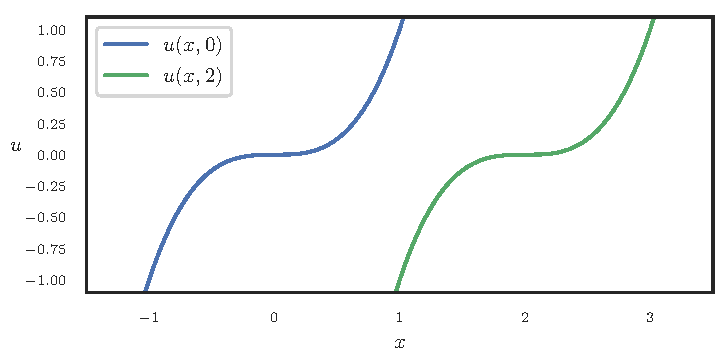
\includegraphics[width=0.75\textwidth]
                  {../images/curved-mesh/simple_transport.pdf}
  \centering
  \caption{The solution to \(u_t + u_x = 0, \; u(x, 0) = x^3\) plotted in
    the \(xu\)-plane. Demonstrates simple transport of
    the solution.}
  \label{fig:simple-transport}
\end{figure}

Motivated by this, \textbf{Lagrangian methods} treat each point in the
physical domain as a ``particle'' which moves along a characteristic curve
over time and then monitor values associated with the particle (heat / energy,
velocity, pressure, density, concentration, etc.). They are an effective way
to solve PDEs, even with higher order or non-linear terms.
For example, if we add a viscosity term to~\eqref{eq:simple-transport}
\begin{equation}
u_t + c u_x - \eps u_{xx} = 0
\end{equation}
then the same characteristics can be used, but the value
along each characteristic is no longer constant; instead it satisfies the
ODE \(\frac{d}{dt} u(x(t), t) = \eps u_{xx}\).

\begin{figure}
  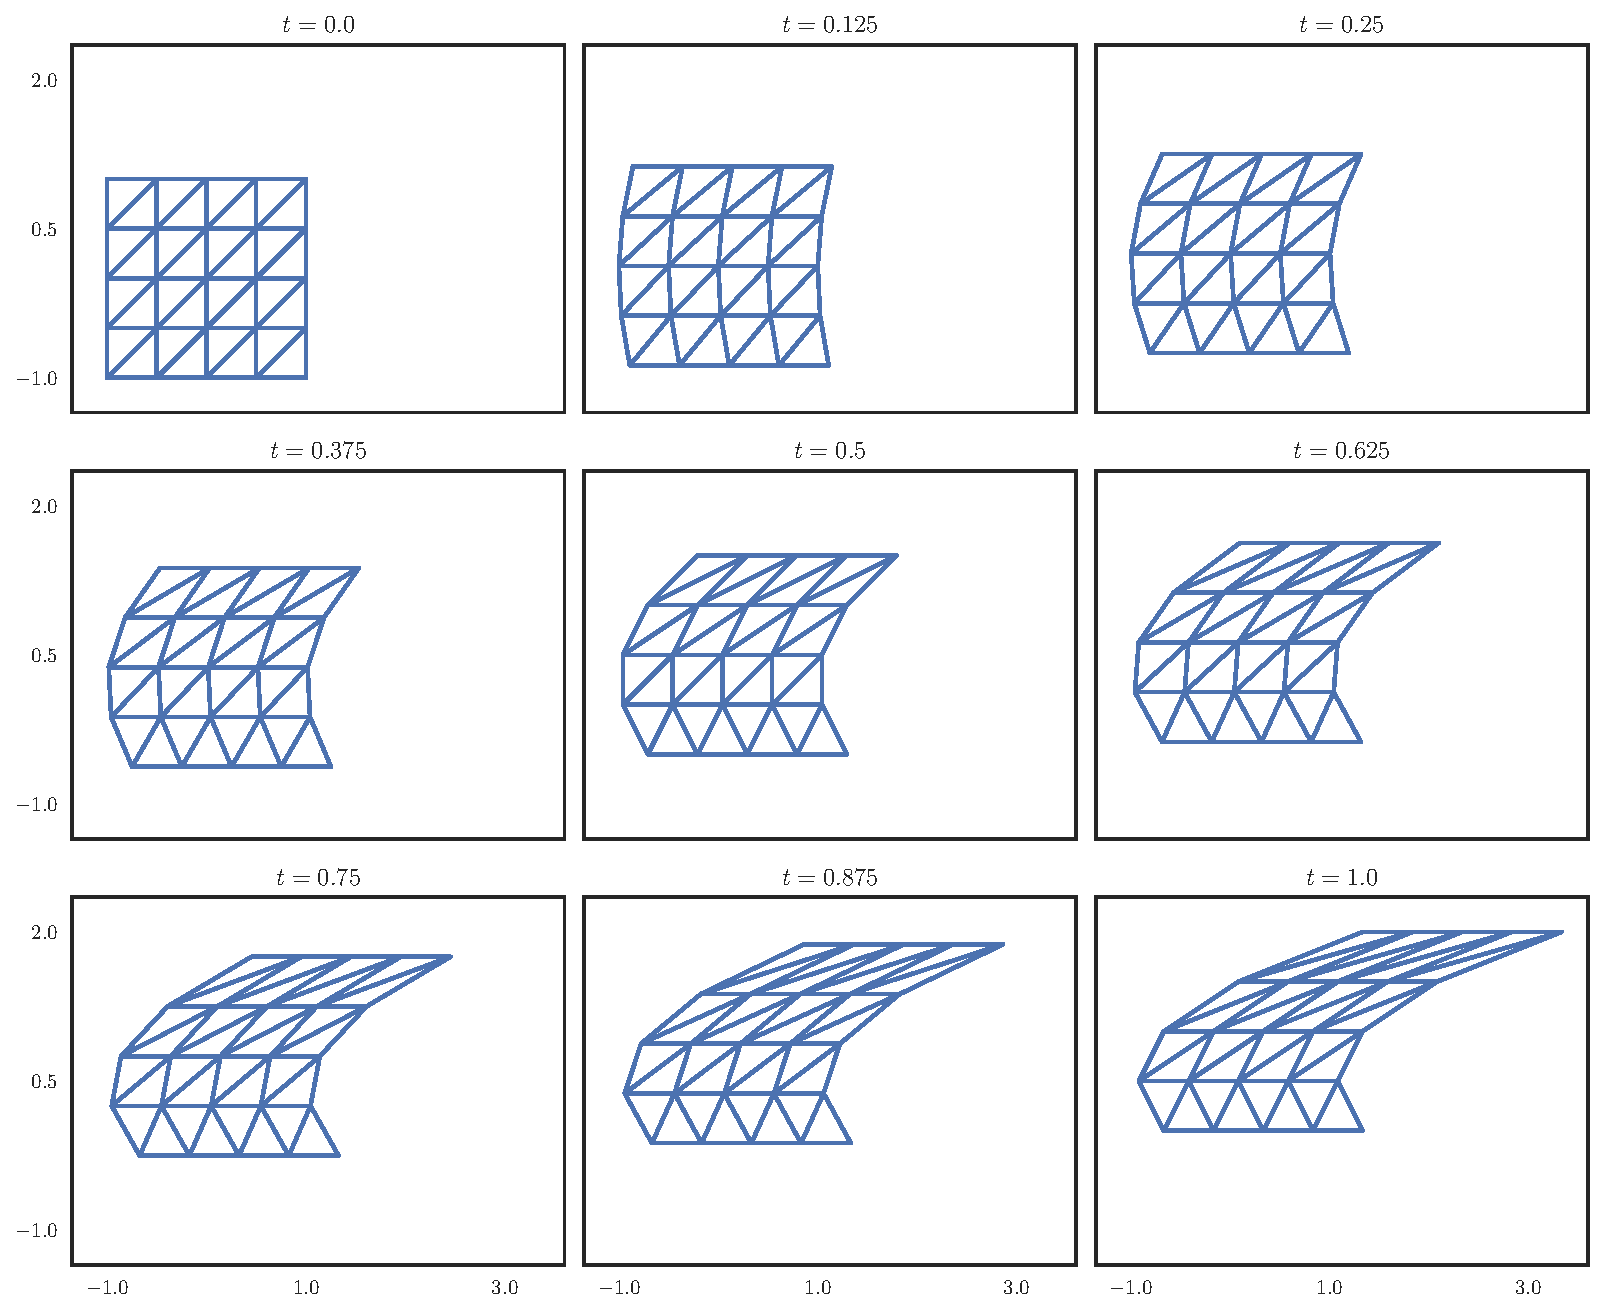
\includegraphics{../images/curved-mesh/mesh_distortion.pdf}
  \centering
  \caption{Distortion of regular mesh caused by particle motion along
    the velocity field \(\left[ y^2 \; 1 \right]^T\) from \(t = 0\)
    to \(t = 1\) with \(\Delta t = 1/4\).}
  \label{fig:mesh-distortion}
\end{figure}

This approach transforms the numerical solution of PDEs into a family of
numerical solutions to many independent ODEs. It allows the use of familiar
and well understood ODE solvers. In addition, Lagrangian methods often
have less restrictive conditions on time steps than Eulerian
methods\footnote{In Eulerian methods, the mesh is fixed.}.
When solving PDEs on unstructured meshes
with Lagrangian methods, the nodes that determine the mesh move (since they
are treated like particles) and the mesh ``travels''. However, mesh changes
can cause problems if it causes the mesh to leave the domain being
analyzed or if it distorts the mesh until the element quality is too low
in some mesh elements.
For an example of such distortion (Figure~\ref{fig:mesh-distortion}),
consider a PDE of the form
\begin{equation}
u_t + \left[ \begin{array}{c} y^2 \\ 1 \end{array}\right] \cdot \nabla u +
  F\left(u, \nabla u\right) = 0.
\end{equation}
The characteristics \(y(t) = y_0 + t, x(t) = x_0 +
\left(y(t)^3 - y_0^3\right)/3\)
distort the mesh considerably after just one second.

Adaptive: \cite{Dukowicz1987, Babuska1978}, Data transfer:
\cite{Jiao2004, Farrell2009, Farrell2011} (In many applications, the field
must be conserved for physical reasons,
e.g. mass or energy cannot leave or enter the system),

%% Excerpt from DK87
%% Traditionally, numerical fluid dynamics has taken the form of
%% Lagrangian or Eulerian methods. Lagrangian methods, in which the computational
%% mesh travels with the fluid, are ideal for the many problems which involve interfaces
%% between materials or free surfaces. However, multidimensional Lagrangian calculations
%% can typically be carried out for only a limited time before severe mesh distortion, or
%% even mesh tangling, destroys the calculation. Eulerian methods, in which the mesh is
%% fixed, are ideal for flows with large deformation but the sharp resolution of interfaces
%% or free surfaces is lost.

%% Excerpt from Iske+Kaser
%% However, in order to balance the method's approximation quality and its computational costs
%% effectively, adaptivity is an essential requirement, especially when modelling multiscale phenomena

%% Excerpt from Jiao+Heath
%% While the comparisons are
%% performed with matching geometries, this paper also addresses additional complexities associated with
%% non-matching surface meshes

%% SUPERMESH == ``common refinement''

%% b is the load vector, M is the mass matrix; Mx = b

%% A limitation of the common-refinement-based approach is that the geometry
%% of the source and target meshes in principle should discretize the same geometry, and some
%% applications may involve partially overlapping meshes

%% Solve PDE / construct S(t) that approximates INT f(x, t) dx: https://doi.org/10.1137/0915051
%% Solve PDE on overlapping 2D meshes: https://doi.org/10.1137/S0036142997323582
%% Solve PDE on overlapping 2D meshes (e.g. if during refinement): https://doi.org/10.1137/0724063

%% However, the basis functions of the donor mesh
%% are (in general) discontinuous piecewise polynomials over any given
%% element of the target mesh, which are very difficult to integrate
%% by numerical quadrature schemes.

%% B\'{e}zier curves and triangles were selected for defining
%% mesh elements for two main reasons. Firstly, using
%% curved instead of linear elements allows us to use
%% meshes with far fewer elements, both for representing
%% geometry and for obtaining accurate numeric solutions.
%% Secondly, B\'{e}zier curves and triangles have a
%% number of mathematical properties leading to elegant
%% algorithms.

%% B\'{e}zier curves are completely defined by their control
%% points which form the control polygon. Similarly,
%% B\'{e}zier triangles are completely defined by their control
%% points which form a control net. See Figure 1.
%% For more information about B\'{e}zier curves and triangles
%% see [11, 12] among others.

%% Since adapting the mesh changes the domain for \(\bm{f}\), we
%% must project \(\bm{f}\) onto the new mesh domain. This is
%% accomplished by making local projections of \(\bm{f}\) whenever
%% local mesh modifications are made, and then computing
%% the local reinterpolation error. The choice of a
%% relevant error norm and projection is problem dependent,
%% but the computations are generally easy, since
%% they are done in a local setting with few degrees of
%% freedom. If the calculated re-interpolation error due
%% to a mesh modification is too great, then the modification
%% can be aborted and can be replaced with a mesh
%% refinement.

\begin{figure}
  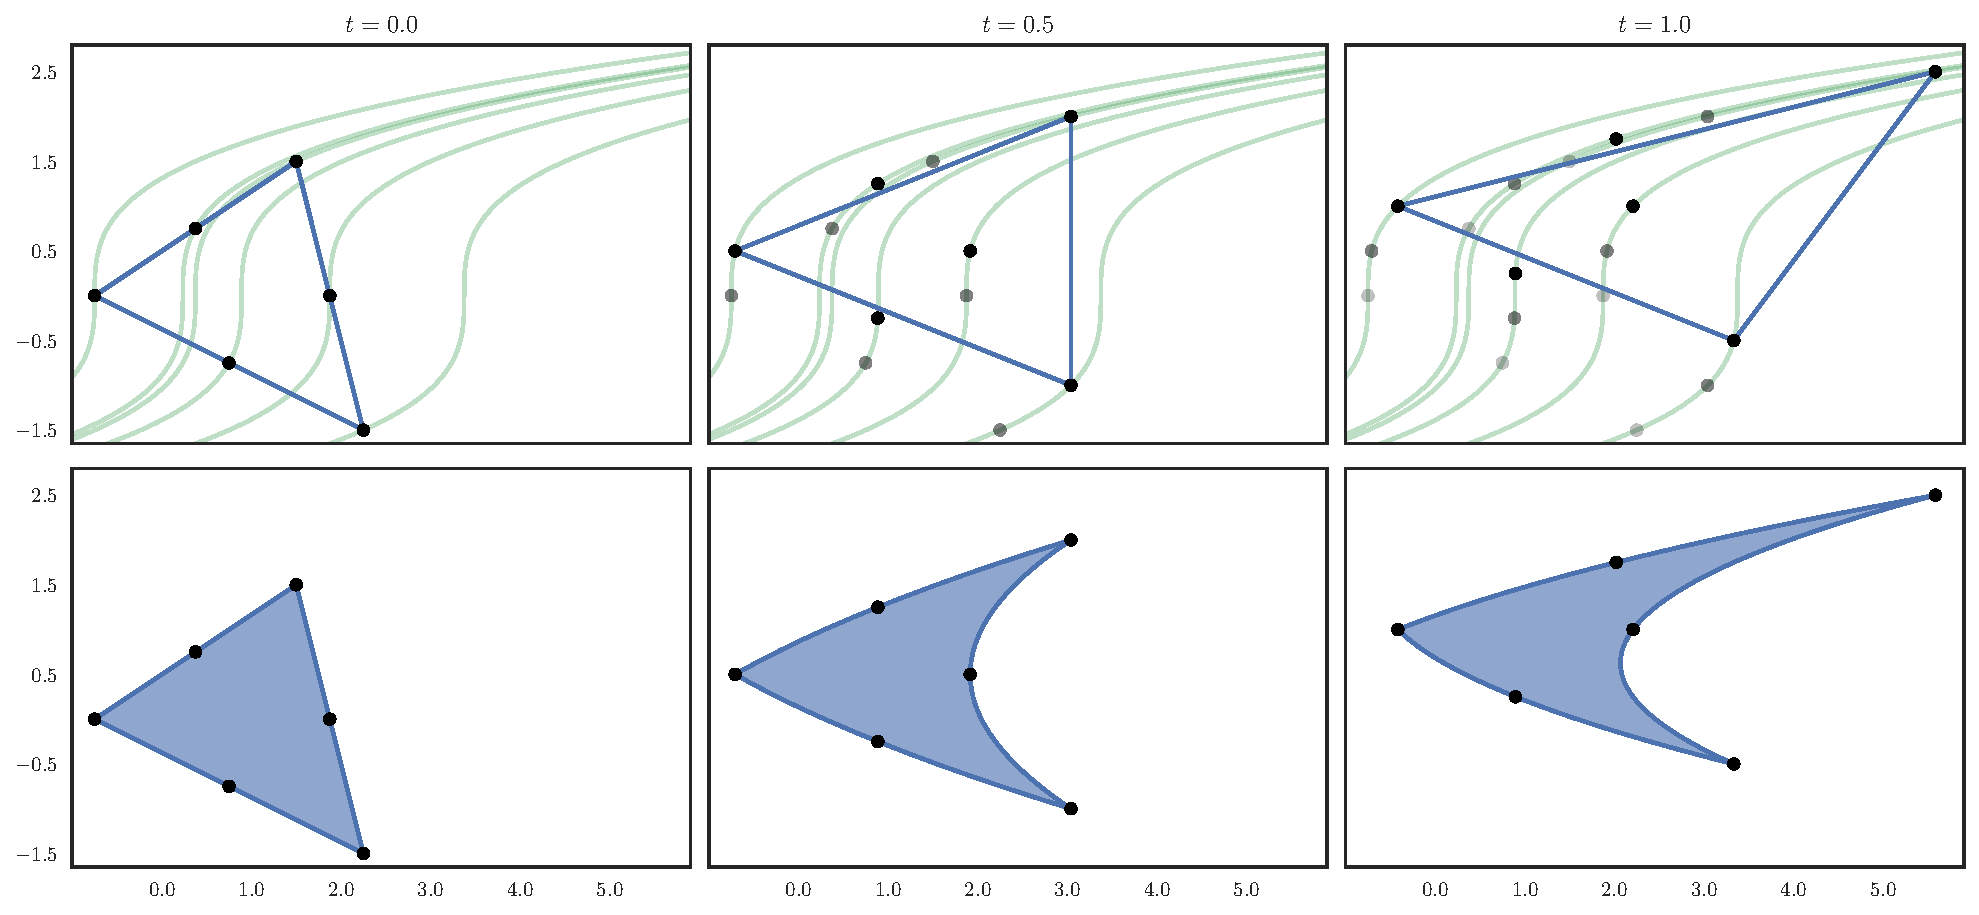
\includegraphics[width=0.9375\textwidth]
                  {../images/curved-mesh/element_distortion.pdf}
  \centering
  \caption{Movement of nodes in a quadratic element under distortion caused
    by particle motion along the velocity field \(\left[ y^2 \; 1 \right]^T\)
    from \(t = 0\) to \(t = 1\) with \(\Delta t = 1/2\).}
  \label{fig:element-distortion}
\end{figure}

\begin{figure}
  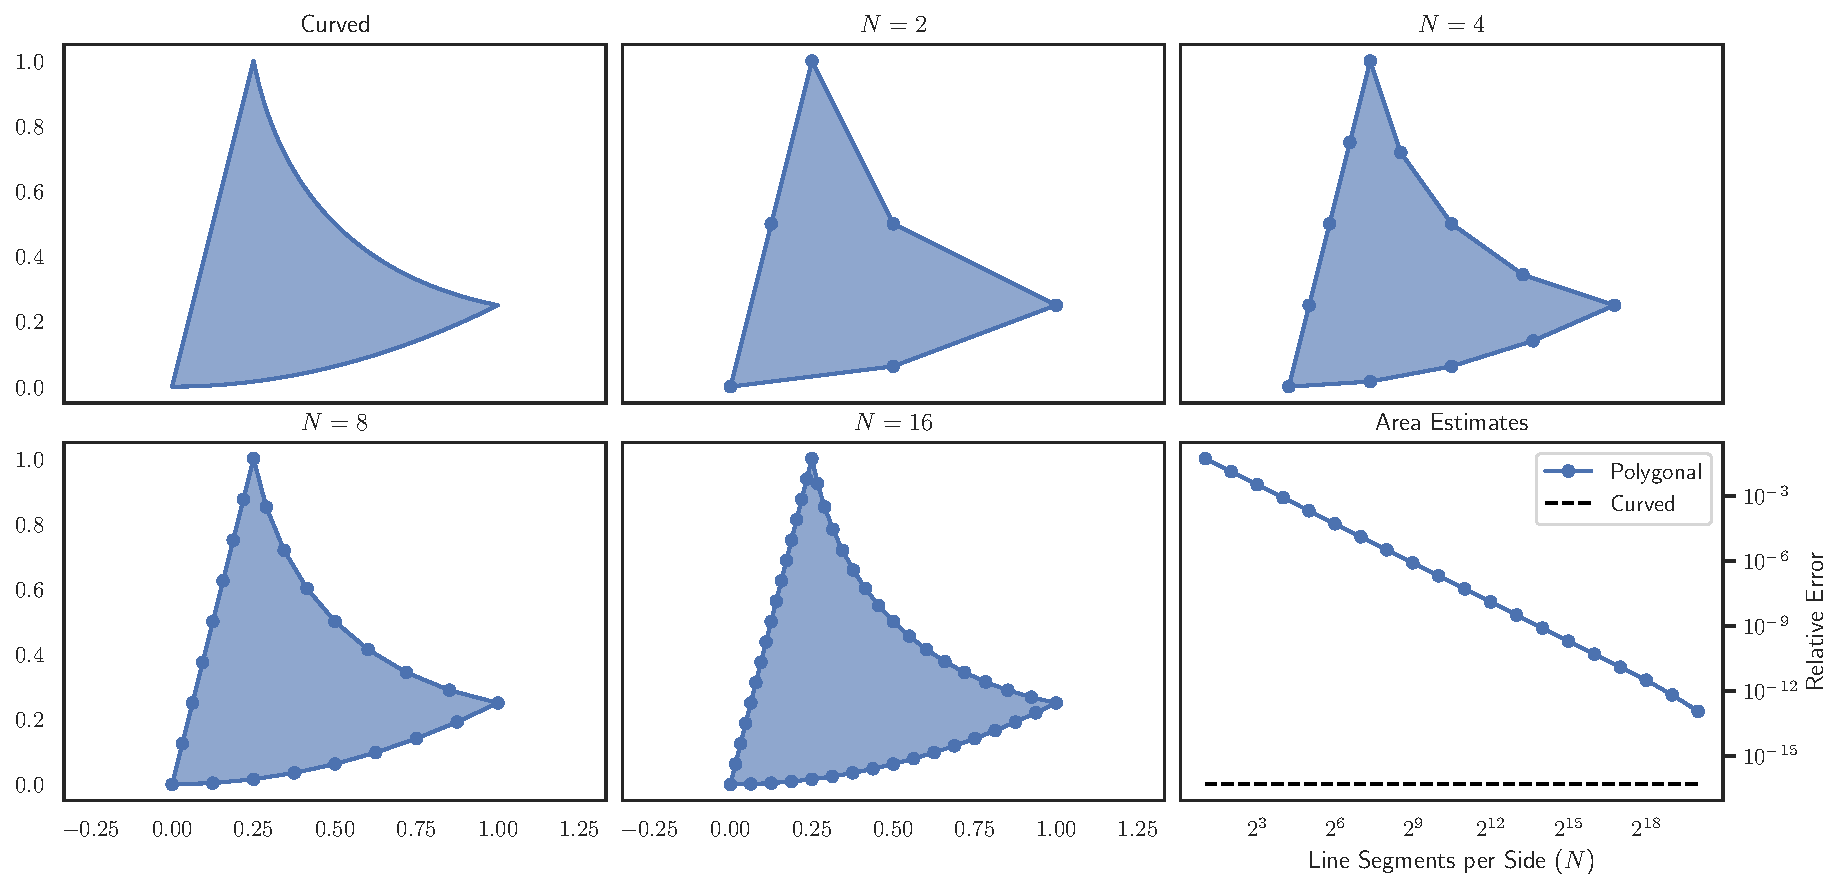
\includegraphics[width=0.9375\textwidth]
                  {../images/curved-mesh/polygon_vs_curved.pdf}
  \centering
  \caption{Comparing the relative error for the computed area of a quadratic
    B\'{e}zier triangle. In one method, the curved boundary is used with
    Green's method and it is correct to machine precision. In the other,
    the curved edges are approximated by polygonal paths. These paths are
    generated from equally spaced parameters, for example a B\'{e}zier curve
    \(b(s)\) with \(N = 4\) would be approximated by a line connecting
    \(b(0), b(1/4), b(1/2), b(3/4)\) and \(b(1)\).}
  \label{fig:polygon-vs-curved}
\end{figure}

\begin{figure}
  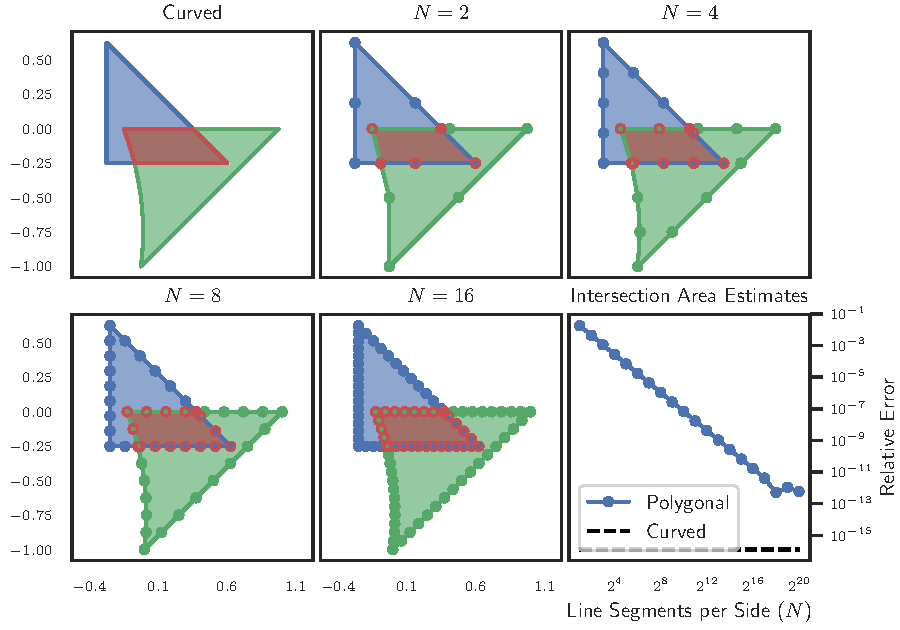
\includegraphics[width=0.9375\textwidth]
                  {../images/curved-mesh/polygon_vs_curved_intersection.pdf}
  \centering
  \caption{Comparing the relative error for the computed area of the
    intersection of two quadratic B\'{e}zier triangles. In one method, the
    intersection boundary is fully specified as the union of B\'{e}zier curve
    segments and the area is found via Green's method. This method is correct
    to machine precision. In the other, the curved edges are approximated by
    polygonal paths and the intersection of the resulting polygons is computed.
    These paths are generated from equally spaced parameters, for example a
    B\'{e}zier curve \(b(s)\) with \(N = 4\) would be approximated by a line
    connecting \(b(0), b(1/4), b(1/2), b(3/4)\) and \(b(1)\).}
  \label{fig:polygon-vs-curved-intersection}
\end{figure}

\begin{figure}
  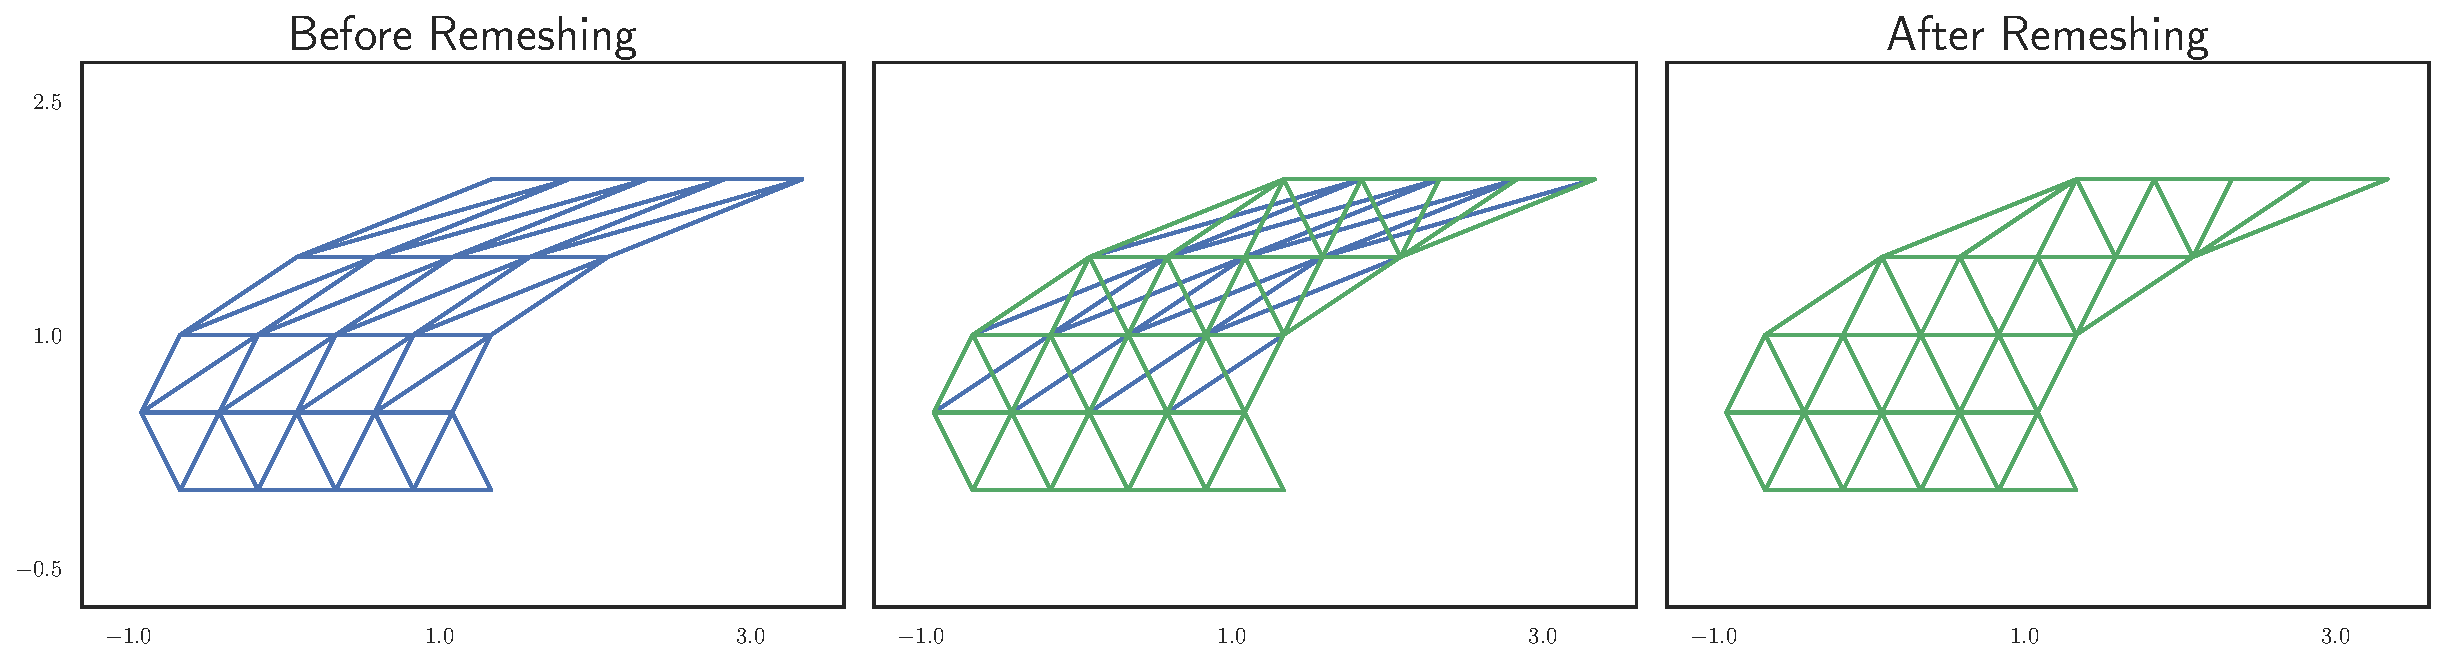
\includegraphics[width=0.9375\textwidth]
                  {../images/curved-mesh/distortion_remesh.pdf}
  \centering
  \caption{Remeshing a domain after distortion caused by particle motion
    along the velocity field \(\left[ y^2 \; 1 \right]^T\) from \(t = 0\)
    to \(t = 1\).}
  \label{fig:distortion-remesh}
\end{figure}

\begin{figure}
  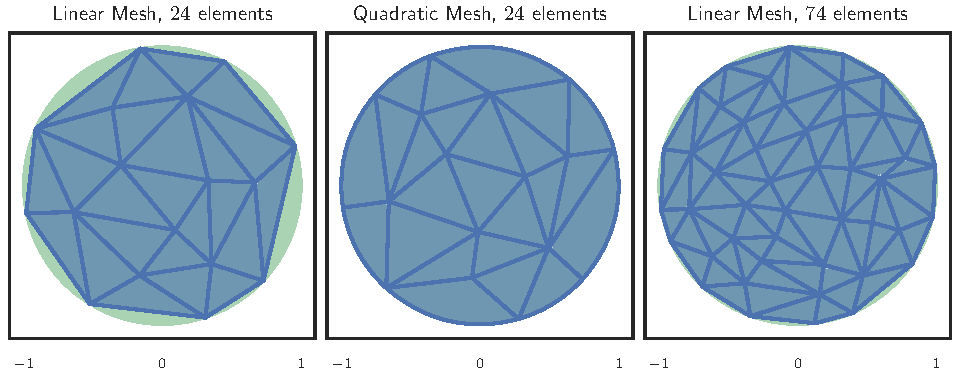
\includegraphics[width=0.9375\textwidth]{../images/curved-mesh/main_figure27.pdf}
  \centering
  \caption{Comparing straight sided meshes to a curved mesh when approximating
    the unit disc in \(\reals^2\).}
  \label{fig:curved-vs-straight-mesh}
\end{figure}

\begin{figure}
  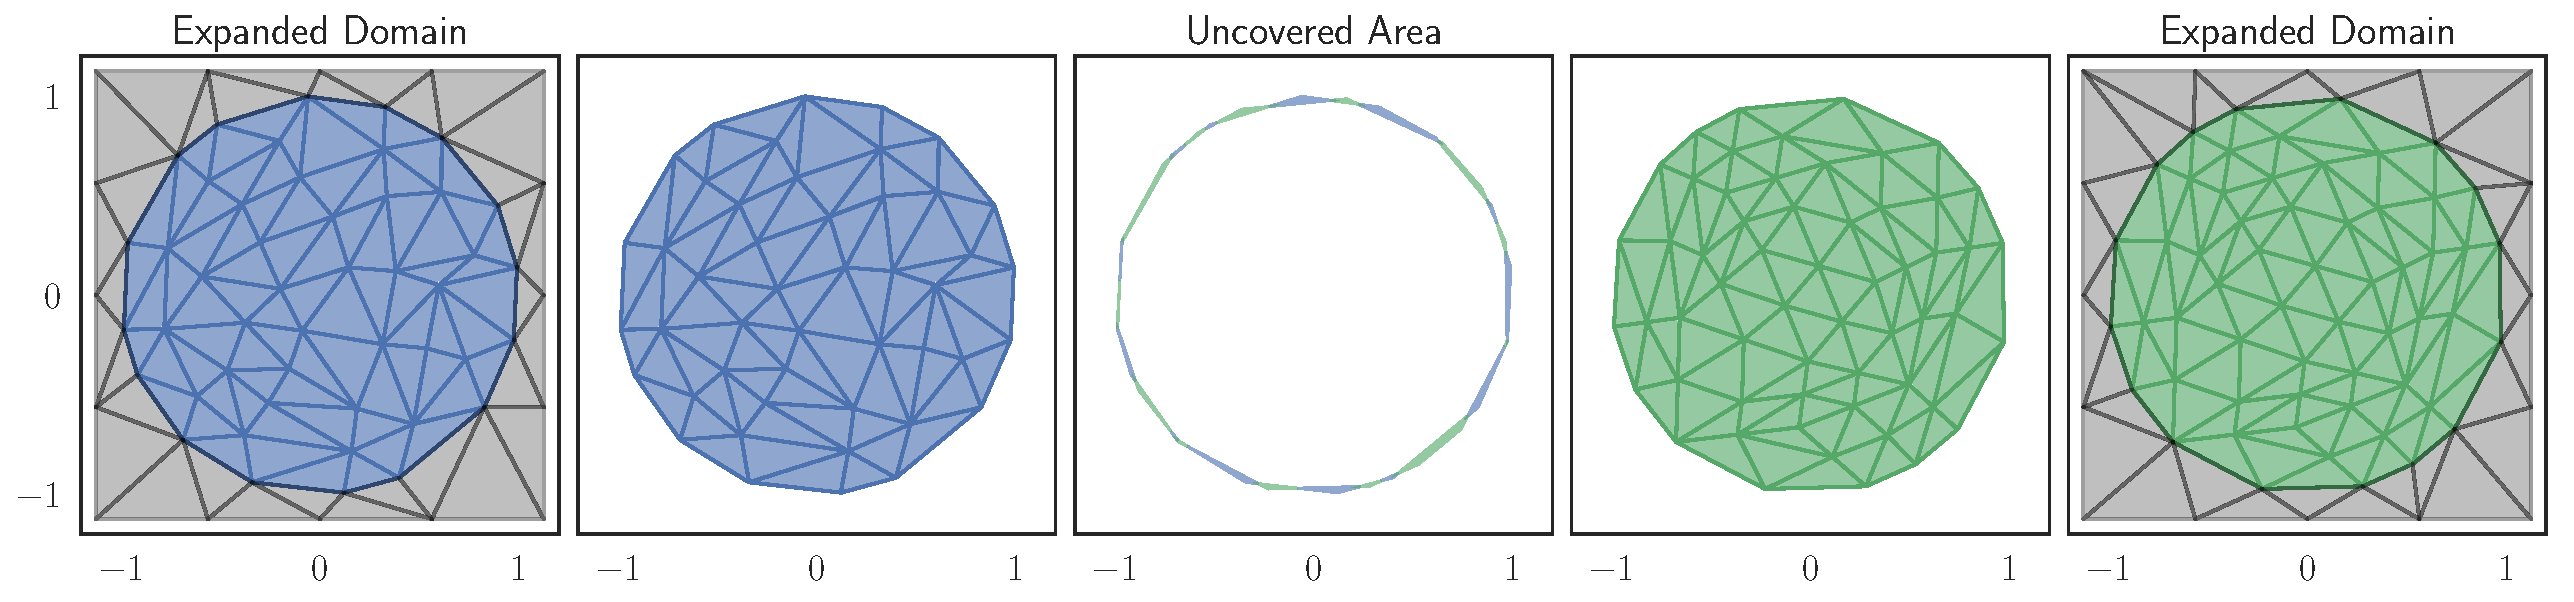
\includegraphics[width=0.96875\textwidth]{../images/curved-mesh/main_figure29.pdf}
  \centering
  \caption{Partially overlapping meshes on a near identical domain. Both are
    linear meshes that approximate the unit disc in \(\reals^2\). The outermost
    columns show how the domain of each mesh can be expanded so they agree.}
  \label{fig:partially-overlapping}
\end{figure}
